\chapter{OBDH with ACS}\label{ch:obdh-acs}

The aim of this assignment is to validate the Attitude Control System (ACS) with Processor In the Loop (PIL). The reduced version of an On-Board Software (OBSW) is used with the ACS of the UPMSat-2 satellite. The ACS uses magnetic sensors and actuators, which is commonly known as magnetic
attitude control (figure~\ref{fig:acs}).

\begin{figure}[h]
            \centering{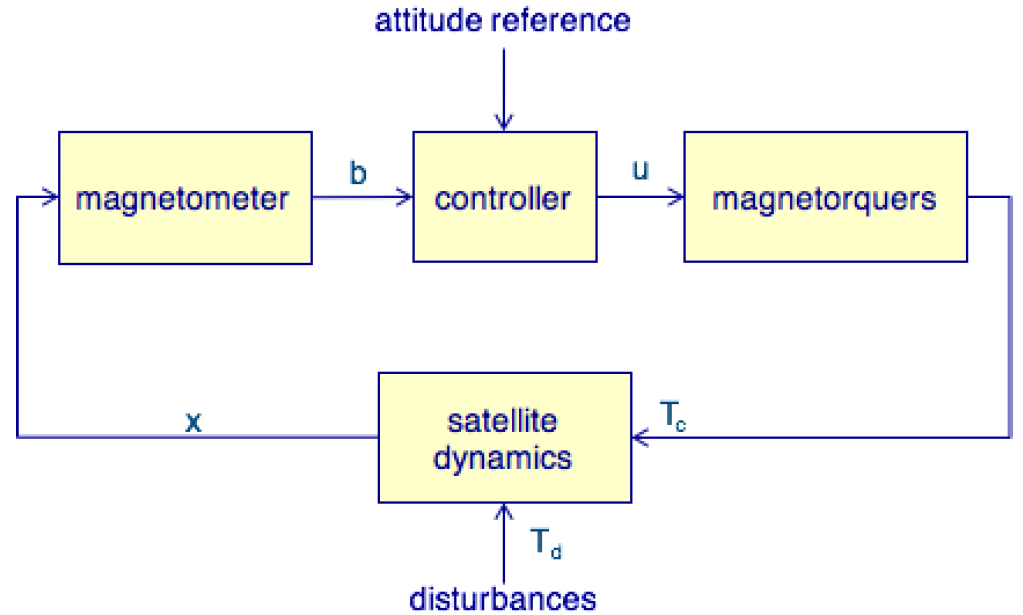
\includegraphics[width=.6\textwidth,keepaspectratio]{acs.png}}
            \caption{Magnetic attitude control system.}
            \label{fig:acs}
\end{figure}

Magnetometers are magnetic sensors that provide a measurement of the strength and direction of the magnetic field, i.e. the magnetic field vector, at a given point. Magnetorquer are magnetic coil which produce a magnetic moment that interacts with the Earth's field, thus enabling the attitude of the satellite to be changed.

\section{Model In the Loop (MIL) validation}

Software validation usually includes testing the system under real operating conditions. However, for obvious reasons, on-board space software as well as many other embedded systems cannot be tested in this way. Simulation models are commonly used in these cases.

The first validation phase uses a model of the ACS, together with models of the space environment and the spacecraft dynamics, to assess the validity of the control law and the design parameters (figure~\ref{fig:acs-hl}). This is usually carried out by a control engineer using a simulation tool. Simulink is commonly used for ACS development.

\begin{figure}[h]
            \centering{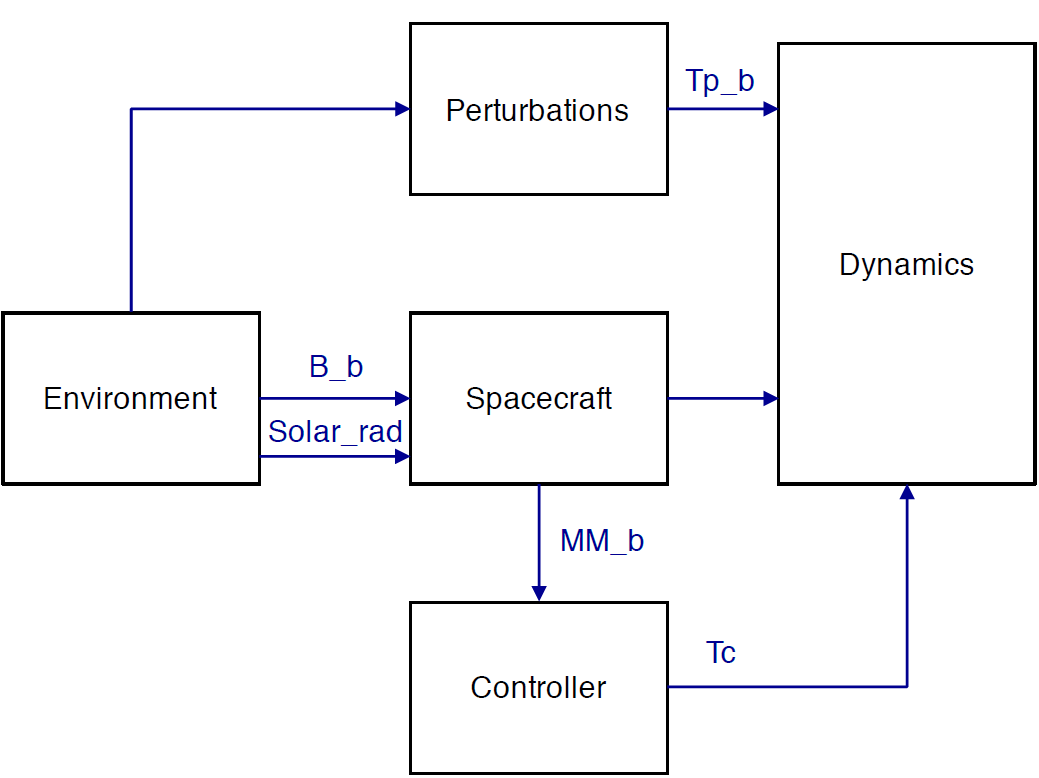
\includegraphics[width=0.6\textwidth,keepaspectratio]{acs-hl.png}}
            \caption{UPMSat-2 ACS high level model view.}
            \label{fig:acs-hl}
\end{figure}

The ACS simulink model can be simulated by running matlab from directory LAB7/ACS and opening ACS.slx. Three new windows will be pop-up: the simulink window with the ACS model and two scope windows that show the angular velocity of the satellite in body reference and the actuation over the three magnetorquers.

The simulink window (figure~\ref{fig:acs-simulink}) shows the high level blocks, that are the satellite itself, its dynamic and the models of the Earth's field and Sun with the perturbations.

\begin{figure}[h]
            \centering{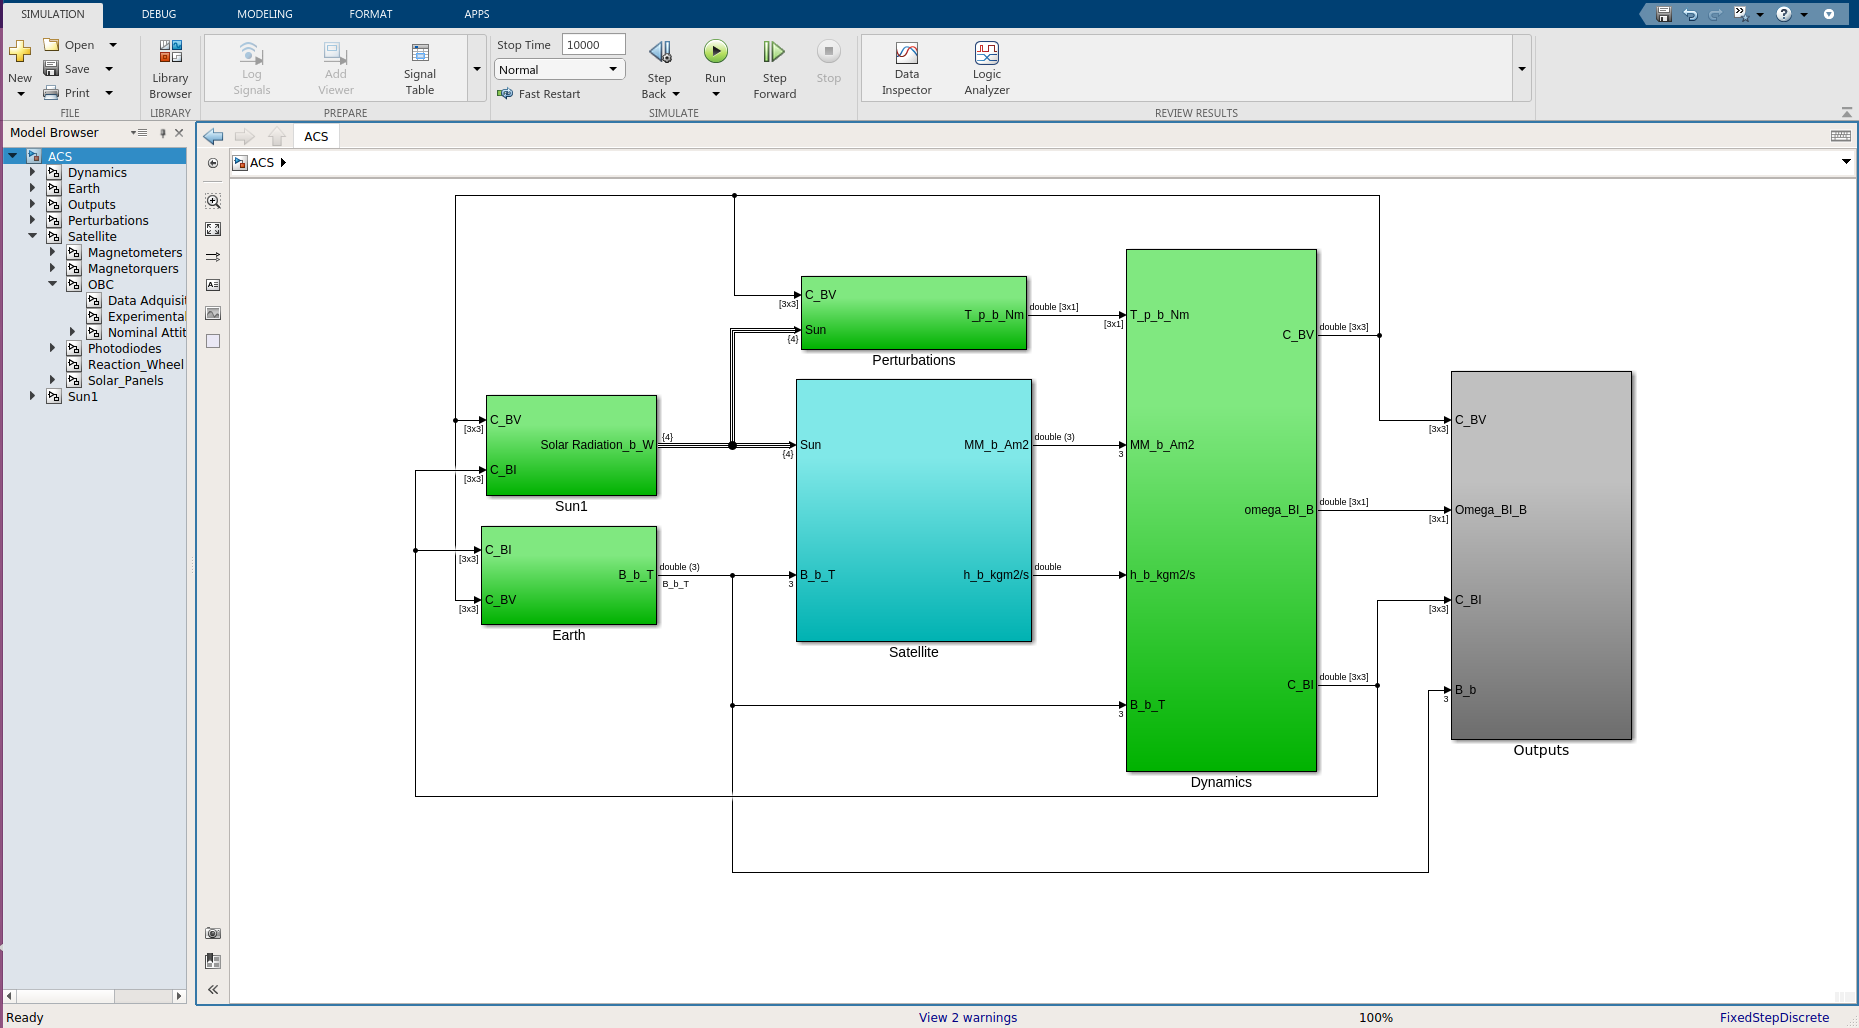
\includegraphics[width=\textwidth,keepaspectratio]{acs-simulink.png}}
            \caption{UPMSat-2 simulink model.}
            \label{fig:acs-simulink}
\end{figure}

The nominal attitude control can be show by selecting Nominal Attitude Control in the Model Browser menu (left part of simulink window) or by clicking on Satellite $\rightarrow$ OBC $\rightarrow$ Nominal Attitude Control blocks.

Nominal attitude control has three blocks (figure~\ref{fig:nac}):
\begin{description}
\item[Sensor] samples the analog inputs of the magnetometers. The inputs are converted to engineering units using calibration data.
\item[Control] implements the attitude control law that computes the control action to be output to the magnetorquers.
\item[Actuator] activates the magnetorquers according to the computed control action.
\end{description}

\begin{figure}[H]
            \centering{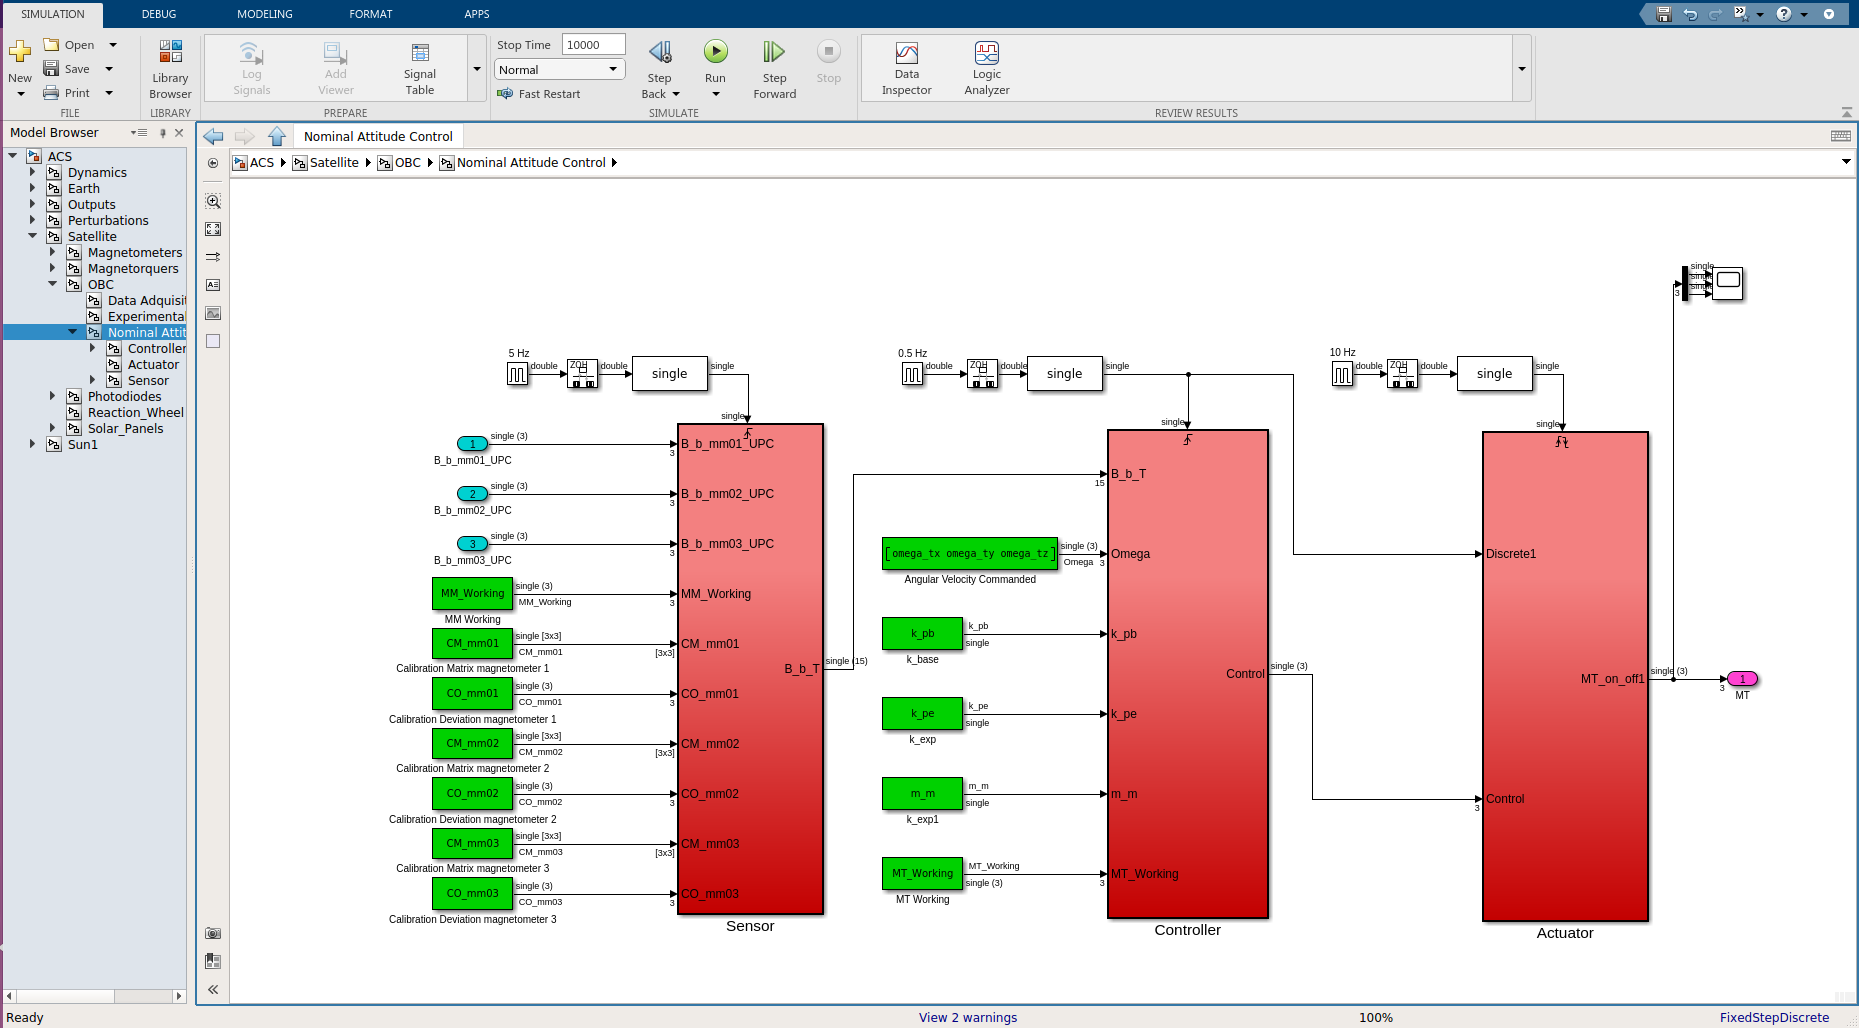
\includegraphics[width=\textwidth,keepaspectratio]{nac.png}}
            \caption{Nominal attitude control.}
            \label{fig:nac}
\end{figure}

To simulate the model an verify its behaviour, click on Run bottom. The evolution of the angular velocity of the satellite and the actuation over the three magnetorquers will be shown in the corresponding scope windows. The commanded angular velocity is [0, 0, 0.1] rad/s and the result of the simulation (figure~\ref{fig:scope}) shows that evolution from the initial angular velocity ([0.1, -0.1, -0.1] rad/s).

\begin{figure}[h]
            \centering{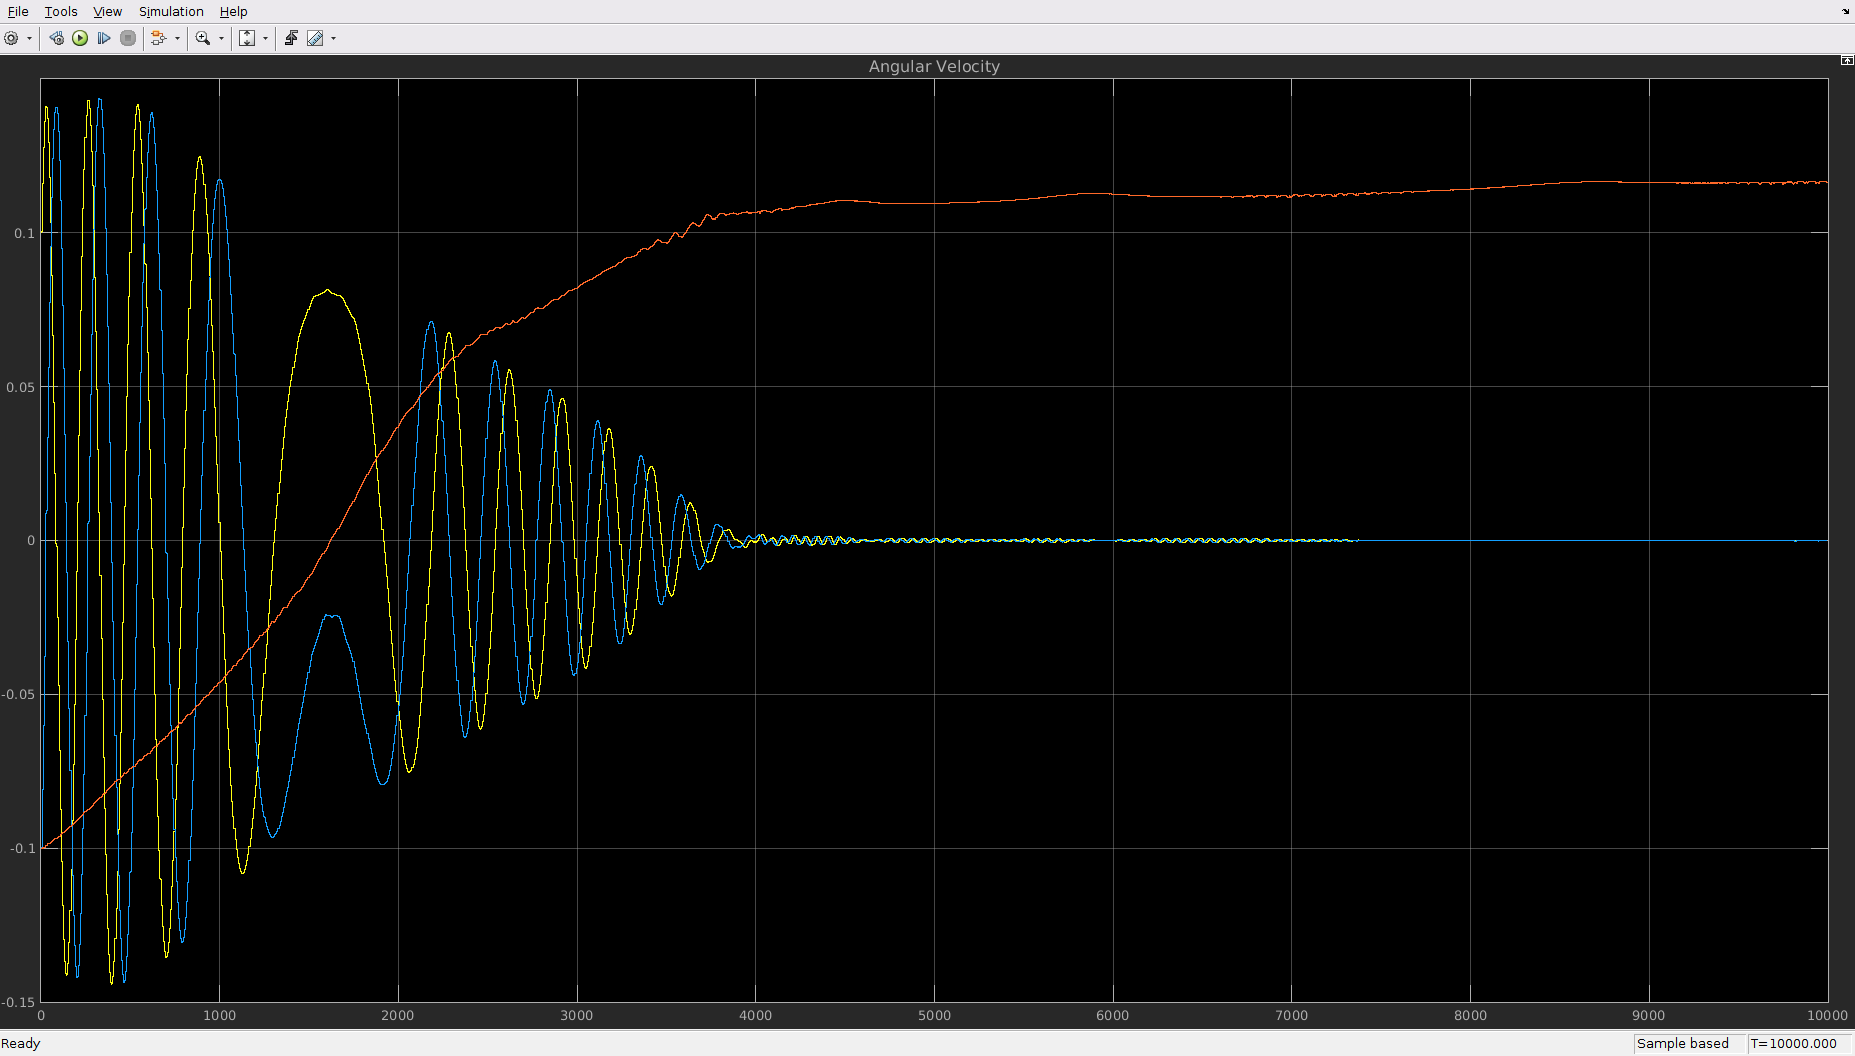
\includegraphics[width=\textwidth,keepaspectratio]{scope.png}}
            \caption{Angular velocity evolution.}

            \label{fig:scope}
\end{figure}

\section{Code generation.}

The next step is execute the ADCS on hardware. In this assignment, only the Control block will be execute on the target board.
The corresponding code can be generated by using the Embedded Coder toolbox but it is needed to isolate Control block from the ACS model. It can be done by clicking in the Control block, selecting all the block content (except the trigger block) and saving it in a new model. 

This model named control.slx can be found in LAB7/ACS\_PIL directory. Use matlab to open it and then select APPS in the top menu, Embedded Coder will appear. If not, it must be installed by clicking Get Add-Ons and searching it. The Embedded Coder window (figure~\ref{fig:control}) will appear after clicking on Embedded Coder icon.

\begin{figure}[h]
            \centering{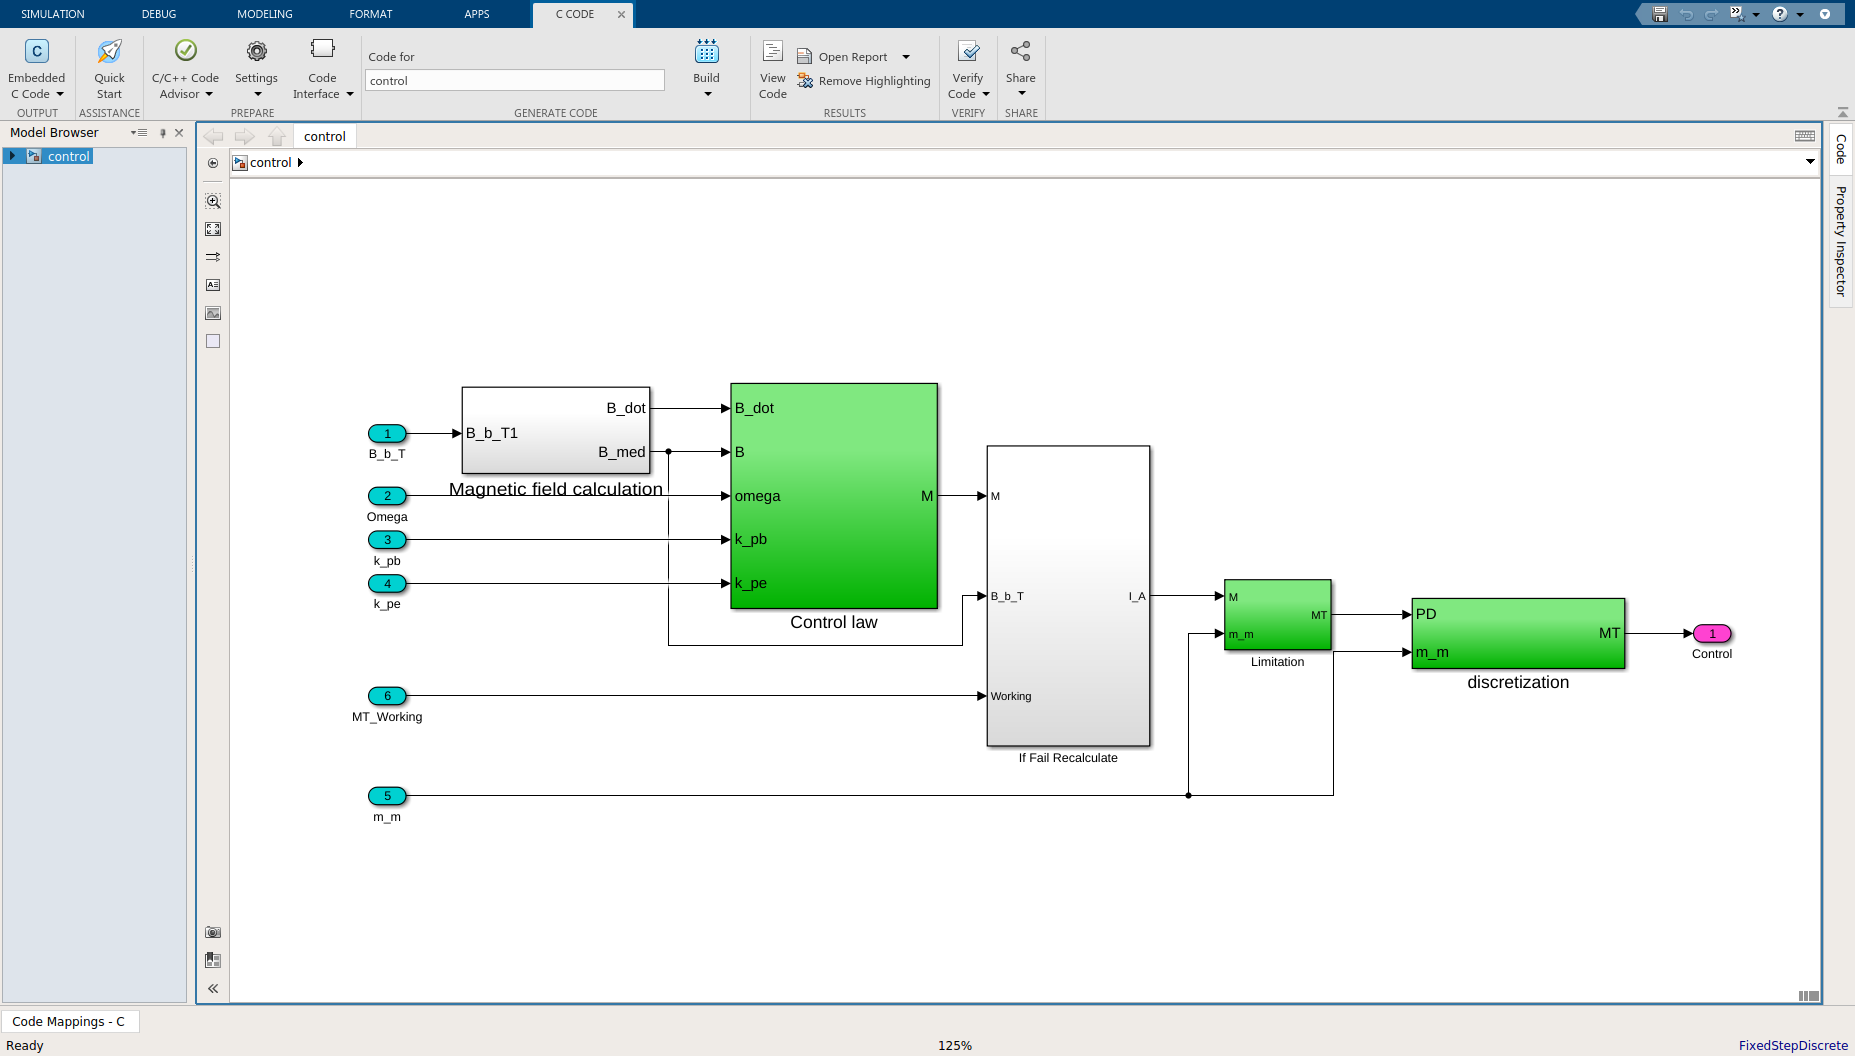
\includegraphics[width=\textwidth,keepaspectratio]{control.png}}
            \caption{Embedded Coder toolbox.}

            \label{fig:control}
\end{figure}

The code generation option as well as characteristics of the target hardware can be set by clicking on the Settings menu. control.slx model has already the proper options, therefore you can take a look but be carefully and do not modify then.

Now the code can be generated by clicking on the Build menu. Once upon the code is generated, a code generation report window appear. It is possible to explore the generated code together with different code metrics. Click on control.h and look for lines 50-79 (figure~\ref{fig:code}) where the generated code interface is located.

\begin{figure}[h]
            \centering{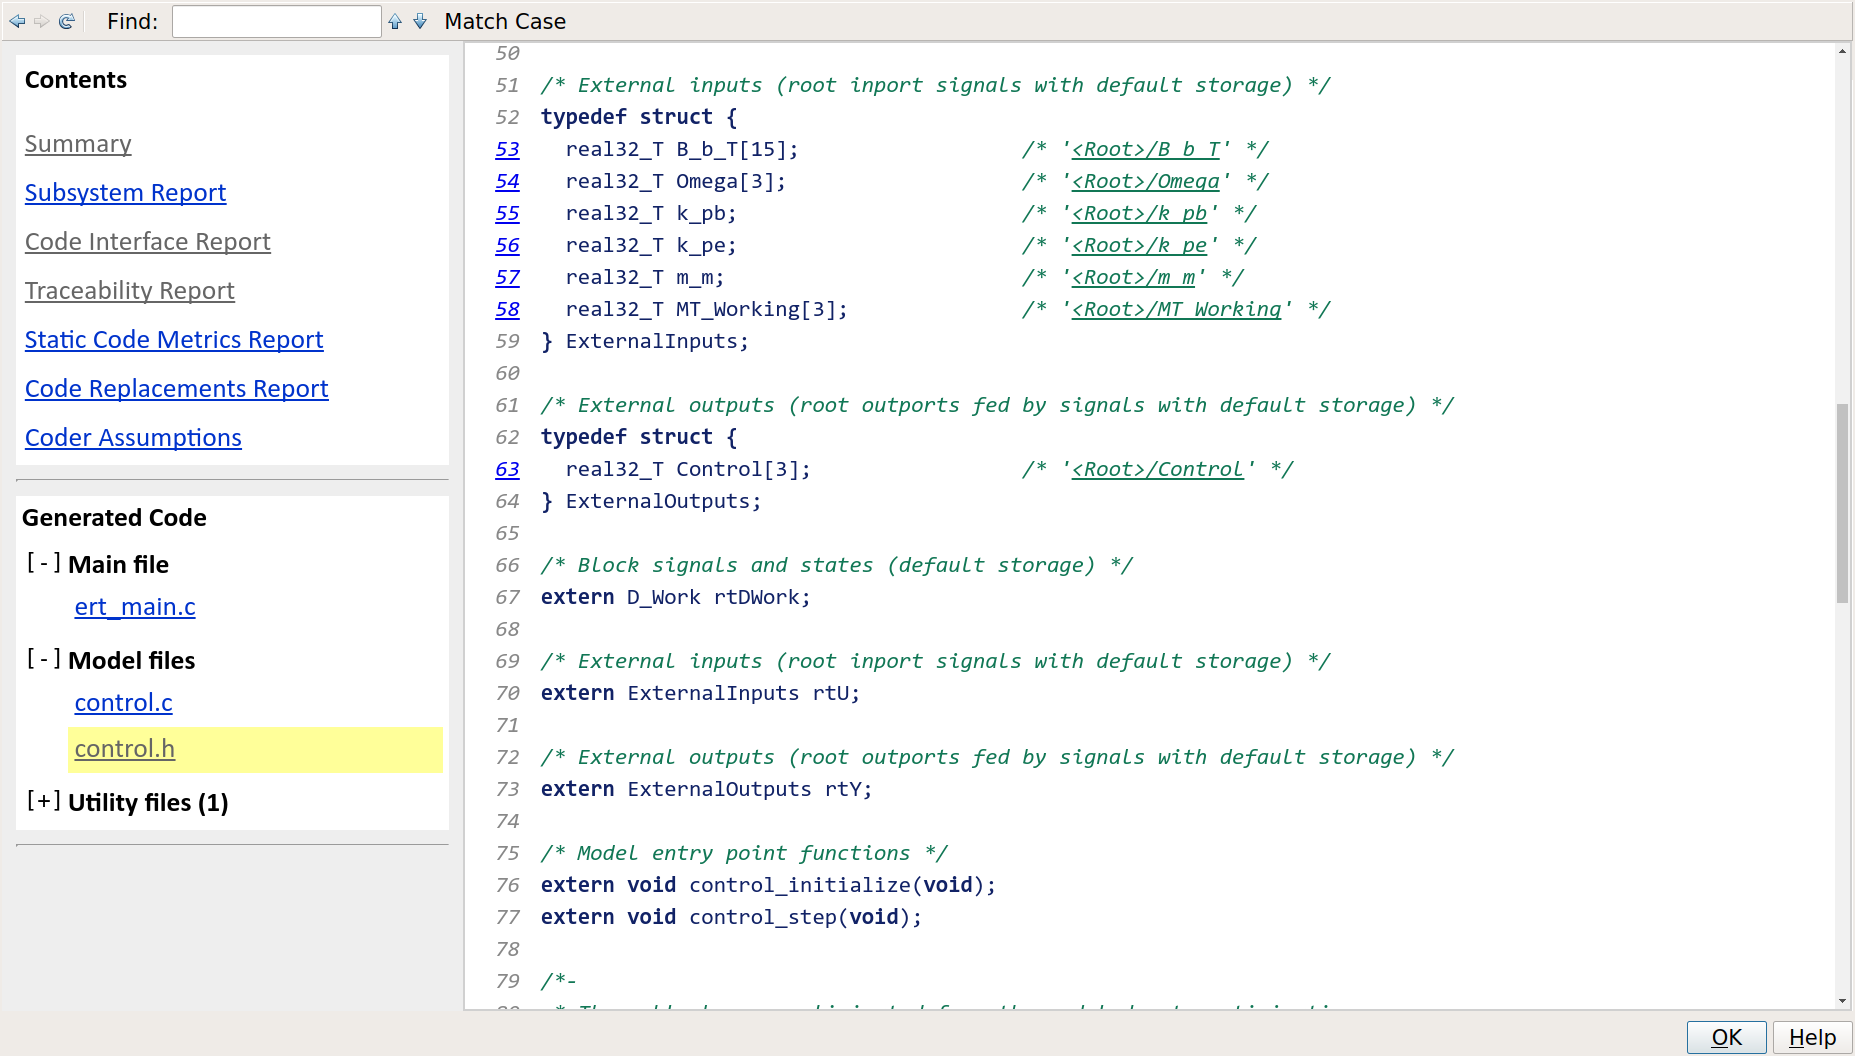
\includegraphics[width=\textwidth,keepaspectratio]{code.png}}
            \caption{Code generation report.}

            \label{fig:code}
\end{figure}

There are two record type definitions (struct) called ExternalInputs and ExternalOutputs that are used to interchange data with the blocks Sensor and Actuator (figure~\ref{fig:nac}). Data are interchanged with two objects: rtU and rtY.
Moreover, function control\_initialize initializes the control code and function control\_step performs the control algorithm.

The generated code will be embedded in the OBSW by taking into account this interface.

\section{Software architecture}

The implementation code, as initially provided to the students, can be downloaded from \url{https://github.com/STR-UPM/SEU-OBDH-Lab/ass-3}.

\begin{figure}[H]
            \centering{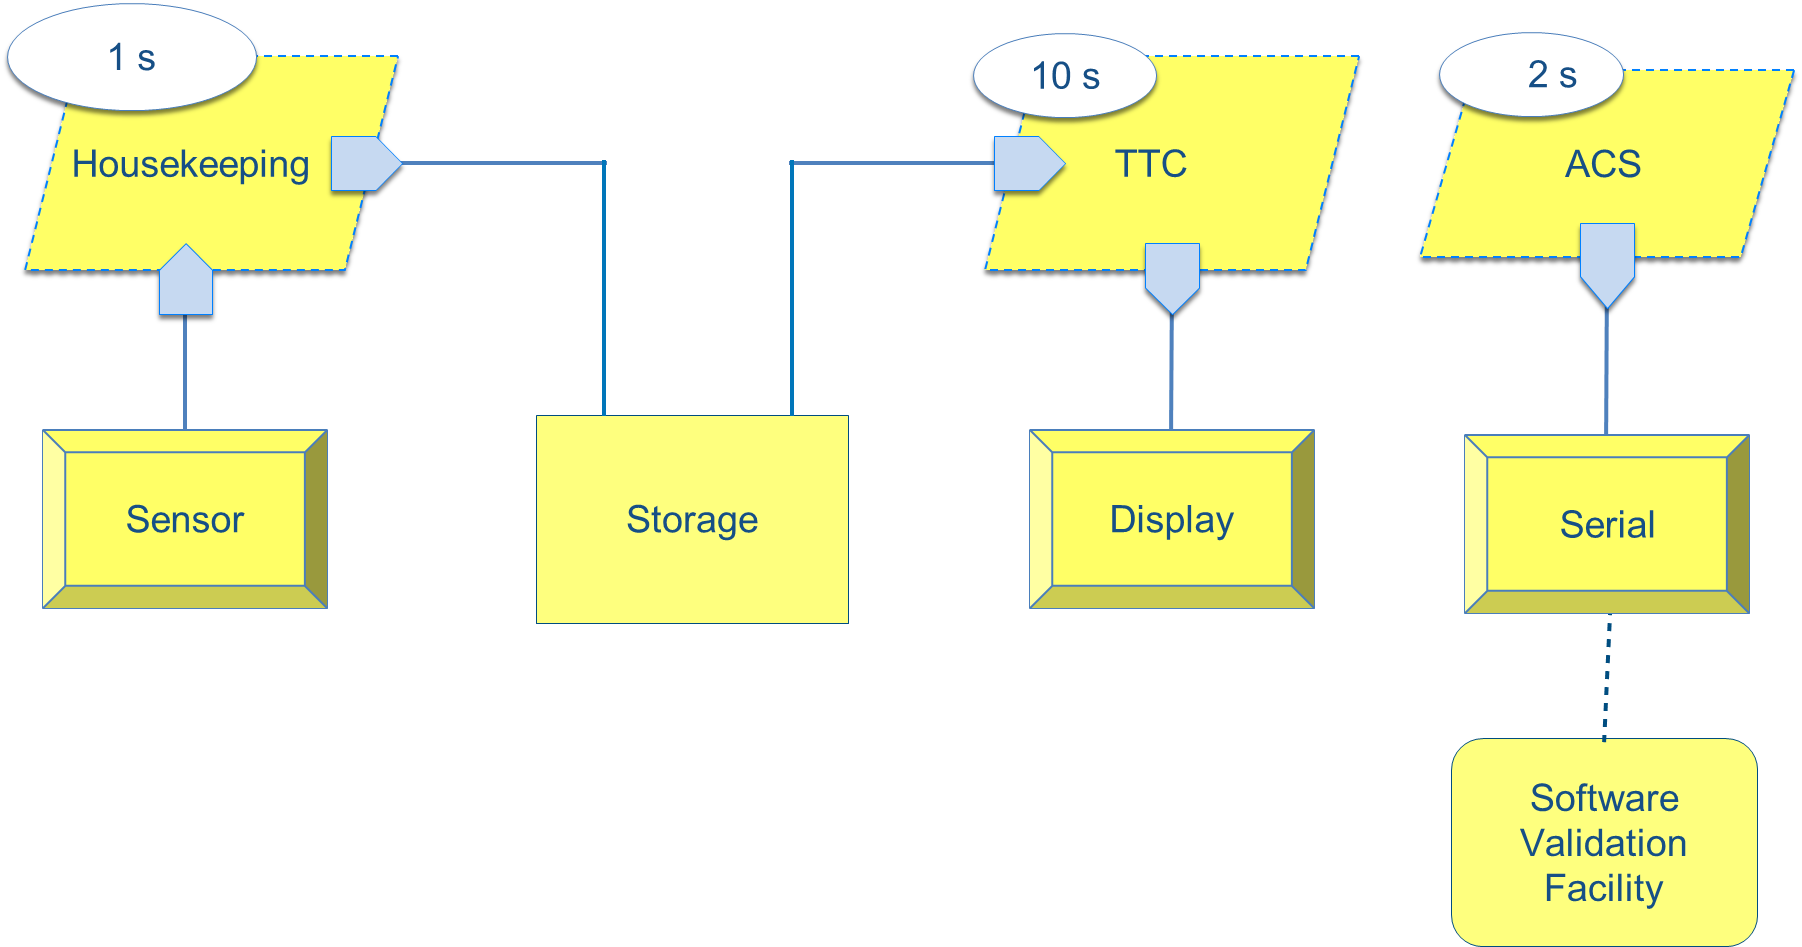
\includegraphics[width=\textwidth,keepaspectratio]{obsw-acs.png}}
            \caption{Software architecture of OBSW with ACS.}
            \label{fig:obdh-acs}
\end{figure}

The software architecture of the OBSW with ACS is depicted in figure~\ref{fig:obdh-acs} and the differences with the previous architecture (figure~\ref{fig:obdh}) are:

The ADCS package is the root element of the ADCS. Its specification consists of one procedure, Initialize, that starts the operation of the component. It has three subpackages:
\begin{description}
\item[ADCS] is the root package of the subsystem and contains a concurrent task, ADCS\_Task that reads the magnetic field vector, calculates the torque vector and sends it to magnetorquers. It also toggles the red LED every two second.

The body of this package uses the generated code by setting the inputs, calling the functions and retrieving the outputs following the interface of figure~\ref{fig:nac}. ADCS\_Task performs the control algorithm by calling control\_step. This is shown in figure~\ref{fig:acs-body}.
It uses Export and Import pragmas to interface the generated C code.

\begin{figure}[h]
            \centering{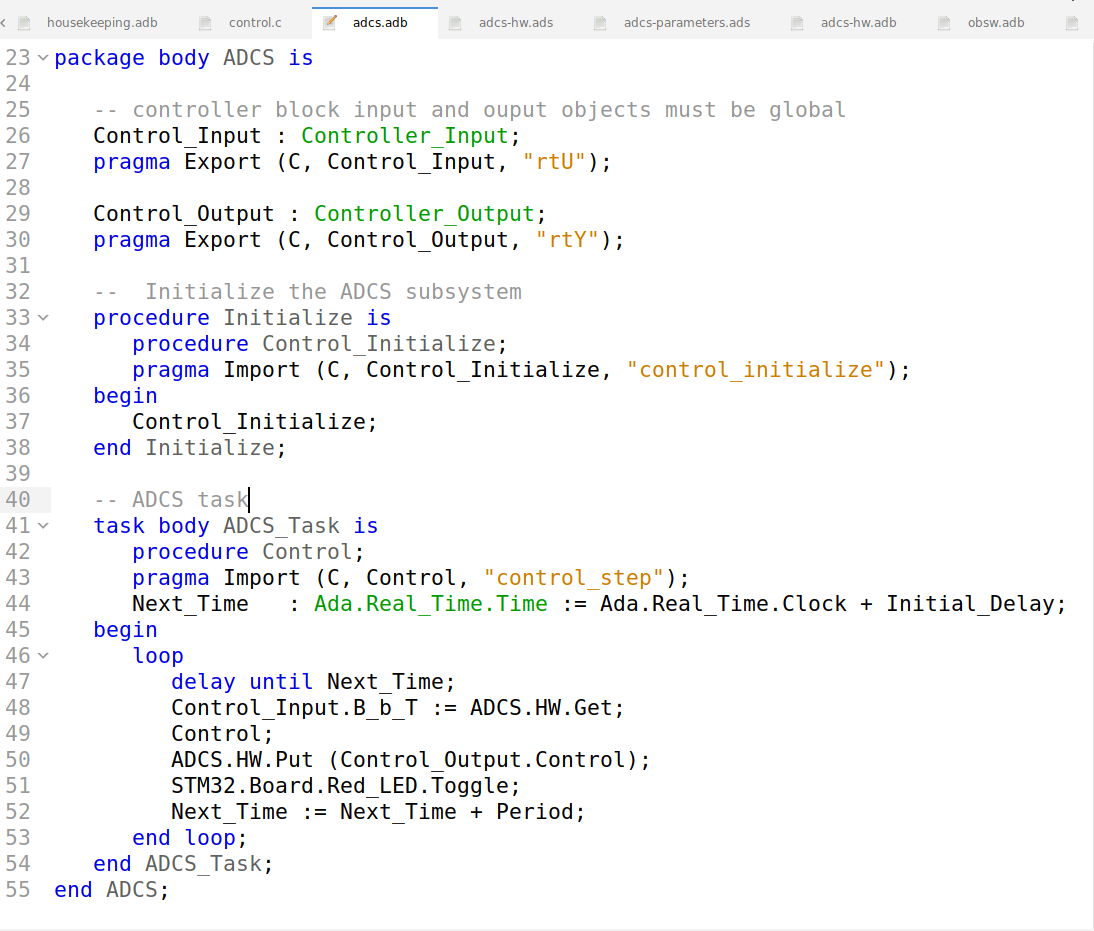
\includegraphics[width=\textwidth,keepaspectratio]{acs-body.png}}
            \caption{Implementation of ACS package.}
            \label{fig:acs-body}
\end{figure}

\item[ADCS.Parameters] contains the definitions of the data types used in the subsystem and parameters that are used to tune the control algorithm. These parameters can be changed by telecommand in the UPMSat-2 OBSW. The data type Controller\_Input is used to read the magnetic field vector in teslas, which are IEEE single precision float numbers. The data type Controller\_Output are used to send the actuation to magnetorquers in newton-meters, which are IEEE single precision float numbers. These data types correspond to the generated C structs ExternalInputs and ExternalOutputs (see figure~\ref{fig:code}).

\item[ADCS.HW] is in charge of getting the magnetic field vector and putting the
torques. It hides the details of the hardware. Its specification includes the Put and Get subprograms. This package uses the serial port to interchange magnetic field and torque values with the Software Validation Facility.
\end{description}

The Software Validation Facility (SVF) is an auxiliary computer, linked to the OBC by a serial line, to run a simulation model of the Earth's magnetic field and satellite dynamics. In this way, engineering values (Nm and T) can be interchanged.

Host computers are also used as SVF by executing a Simulink\texttrademark model of the Earth's magnetic field and satellite dynamics.

In this assignment, the serial line is used to interchange data between ADCS and SVF. Therefore, housekeeping telemetry are send to a text console that is simulated on the host computer, using a mechanism called semihosting. When the target board is connected to the host by means of the ST-LINK USB cable, and the embedded program is run using the debugger in the host, the standard output is re-directed to the debugger console. The GPS environment supports semihosting.

\section{Compile and run with the debugger.}

Open GPS and do the following:
\begin{enumerate}
\item Select Open project on the welcome window. Navigate to the OBSW directory and open the realtime\_housekeeping.gpr project file.
\item Build the executable and load it into the board by clicking on the \hbox{
\includegraphics[width=1.5em]{debug.png}} symbol in the tool bar (or select Build $\rightarrow$ Bareboard $\rightarrow$ Debug on board on the top menu).

The program will be compiled, and the executable will be loaded into the board memory by the debugger. The debugger console (lowest window in GPS) shows the following lines:
\begin{verbatim}
...
(gdb) monitor reset halt
(gdb)
\end{verbatim}

\item Type continue or just c on the debugger console (or select Debug $\rightarrow$ Continue on the top menu).
\begin{verbatim}
(gdb) c
Continuing.
[program running]
\end{verbatim}

After that, the program starts to run on the board and temperature reads are displayed on Messages tab of the debugger window. However, the Red LED does not blink because ACS is waiting sensor inputs from SVF.
\end{enumerate}

\section{Processor In the Loop (PIL) validation.}

The SVF shall provide sensor inputs and retrieve magnetotorquer outputs. To do that, the remain part of the original simulink model will be used, i.e. all the blocks except the Sensor block.

This model named ACS\_PIL.slx can be found in LAB7/ACS\_PIL directory. Open it and again three new windows will be pop-up: the simulink window with the ACS\_PIL model and two scope windows that show the angular velocity of the satellite in body reference and the actuation over the three magnetorquers.

The Control block of this model has been substituted by serial link connections as shown in figure~\ref{fig:nac-pil}. Identify the serial port name on the host computer and edit the serial configuration block by selecting the serial line of your PC.

\begin{figure}[h]
            \centering{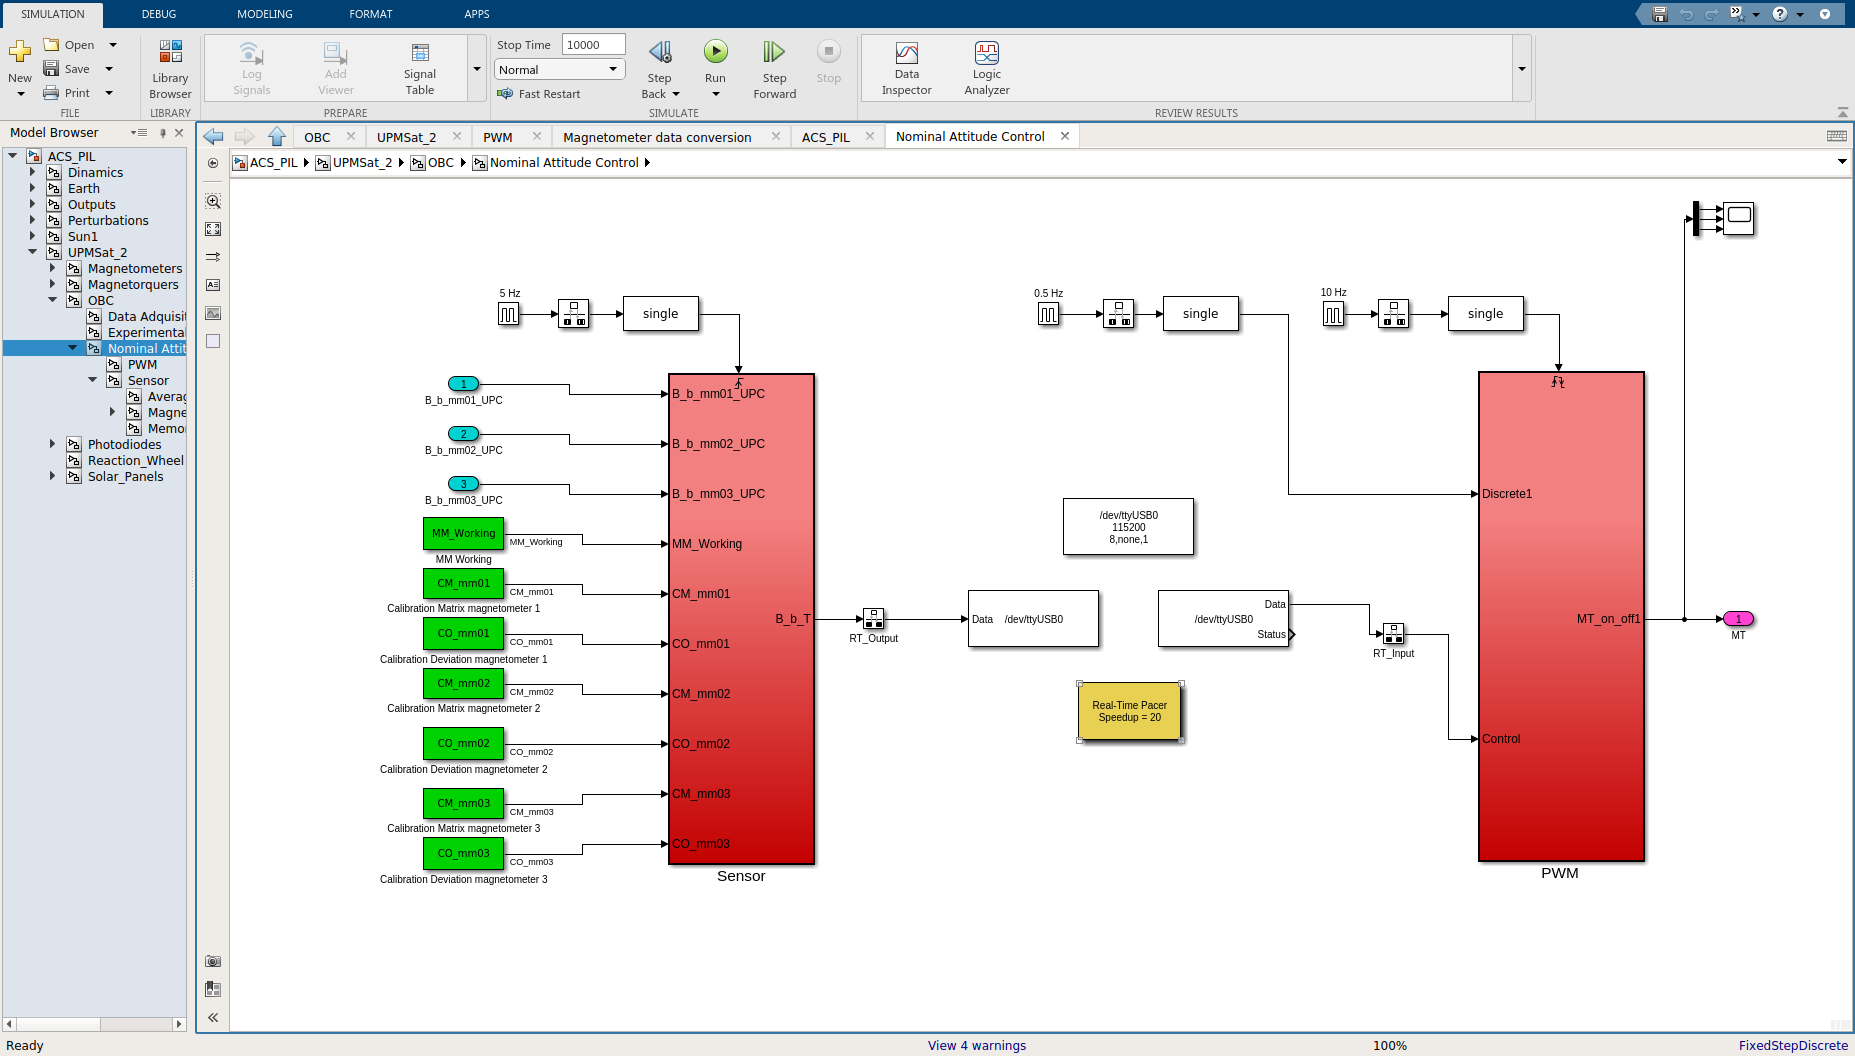
\includegraphics[width=\textwidth,keepaspectratio]{nac-pil.png}}
            \caption{Nominal attitude control for PIL.}
            \label{fig:nac-pil}
\end{figure}

Additional rate transition blocks has been added for a proper communication and a Real-Time Pacer block has been also added to set the simulation speed. In a real case, an speedup equal to 1 should be used but it is to slow.

Start the simulation and verify angular velocity stabilization. Now ADC runs and red LED is toggled. 

\section{Make changes to the simulation.}

\begin{itemize}
\item Default parameters for control blocks can be changed in Ada source file ACS-parameters.ads.
\begin{itemize}
\item Default\_omega is the consigned angular velocity.
\item Default\_MT\_Working contains the operational magneto-torques.
\end{itemize}

In UPMSat-2 many parameters can be changed by TC.
\item The initial angular velocity can be changed in Simulink source file initialization.m.
\begin{itemize}
\item omega\_BI\_B0 = [0.1;-0.1;-0.1];
\end{itemize}
\end{itemize}
